\chapter{Crystallography and X-ray Diffraction}\label{ch:b3:x-ray-diffraction}

In 1912 a beam of X-rays sent through a crystal of copper sulfate left on a
photographic plate a pattern of sharp spots: crystals diffract X-rays as a
grating diffracts light, because the distances between their atoms are
comparable to the X-ray wavelength. A year later William Lawrence Bragg, then a
student, read from such patterns the structure of rock salt --- and showed that
the solid contains no \ce{NaCl} molecules at all, only a lattice in which each ion
has six neighbours of the other kind. Every crystal structure quoted in the
Year 1 volume and in this book was found in this way. This chapter gives the
geometry of lattices and of their symmetry, the condition for diffraction, the
intensities that reveal the contents of the cell, and the powder and
single-crystal methods used in every laboratory.

\begin{recall}
The Year 1 volume described crystals by a lattice of nodes, a motif and a unit
cell with its lattice parameters; counted the multiplicity of a cell; built
the face-centred and body-centred cubic and the hexagonal close-packed
structures and the rock-salt, caesium chloride, zinc-blende and fluorite
types; and computed a density from a cell. \Cref{ch:b3:point-groups} defined
\omterm{def:b3:point-groups:operation}{symmetry operations} and \omterm{def:b3:point-groups:point-group}{point groups}.
\end{recall}

\begin{omfigure}
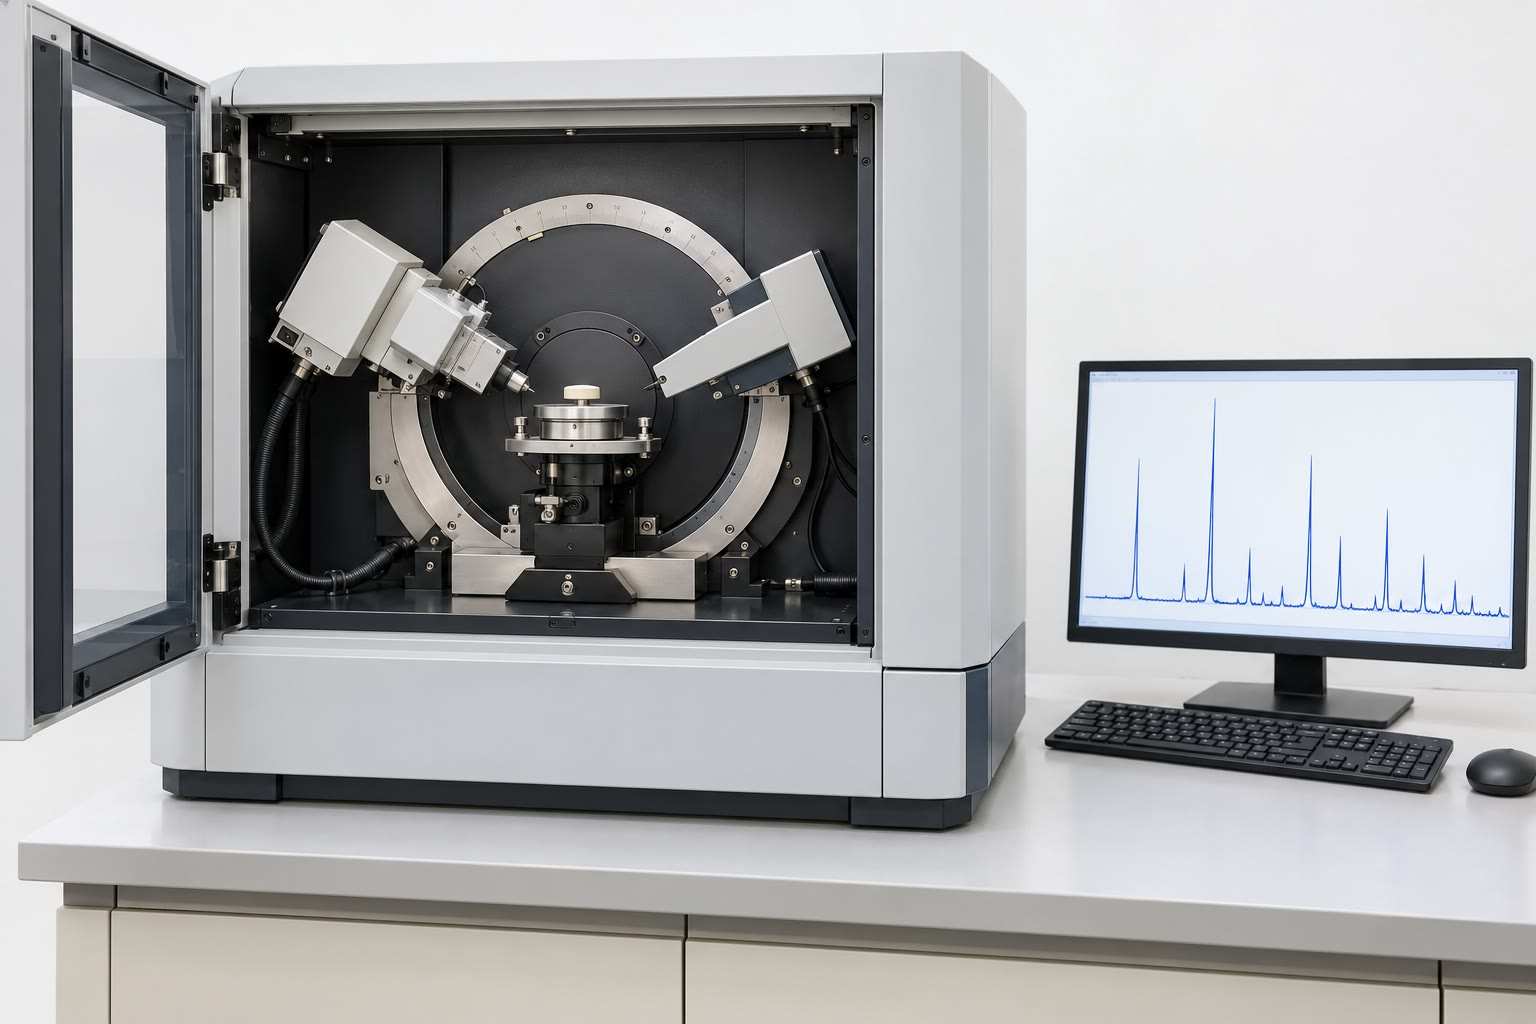
\includegraphics[width=0.6\linewidth]{images/book4/ai/b3-09-diffractometer.jpg}

{\small A benchtop powder diffractometer: the X-ray tube and the detector
turn on a circle around the flat sample.}
\end{omfigure}

\section{Crystal systems and Bravais lattices}

A lattice can only have \omterm{def:b3:point-groups:operation}{symmetry operations} that map the lattice onto itself.
That restricts them severely.

\begin{theorem}[The crystallographic restriction]\label{thm:b3:x-ray-diffraction:restriction}
The only rotation axes compatible with a lattice are of order 1, 2, 3, 4 and 6.
\end{theorem}

\begin{proof}
In a basis of lattice vectors, a symmetry rotation maps lattice vectors onto
lattice vectors, so its matrix has integer entries and an integer trace. The
trace does not depend on the basis; in an orthonormal basis with $z$ along the
axis it is $1 + 2\cos\theta$. Hence $2\cos\theta$ is an integer between $-2$ and 2:
$\cos\theta \in \{-1, -\frac12, 0, \frac12, 1\}$, $\theta = 180^\circ, 120^\circ, 90^\circ,
60^\circ, 0^\circ$: orders 2, 3, 4, 6, 1. A fivefold axis is impossible.
\end{proof}

\begin{definition}[Crystal system, Bravais lattice, lattice centring]\label{def:b3:x-ray-diffraction:crystal-system}
Lattices are grouped by their symmetry into seven \emph{crystal
systems}\index{crystal system} (triclinic, monoclinic, orthorhombic, tetragonal,
trigonal, hexagonal, cubic). A cell may hold lattice nodes only at its corners
(primitive, P) or also at its centre (body-centred, I), at the centres of all
faces (face-centred, F) or of one pair of faces (base-centred, C), or along a
body diagonal (rhombohedral, R): this is its \emph{lattice
centring}\index{lattice centring}. The 14 distinct combinations of a system and
a centring are the \emph{Bravais lattices}\index{Bravais lattice}.
\end{definition}

\begin{center}\small
\begin{tabular}{lll}
\hline
system & cell constraints & centrings \\ \hline
triclinic & none & P \\
monoclinic & $\alpha = \gamma = 90^\circ$ & P, C \\
orthorhombic & $\alpha = \beta = \gamma = 90^\circ$ & P, C, I, F \\
tetragonal & $a = b$, all angles $90^\circ$ & P, I \\
trigonal & $a = b = c$, $\alpha = \beta = \gamma \ne 90^\circ$ (rhombohedral axes) & R \\
hexagonal & $a = b$, $\alpha = \beta = 90^\circ$, $\gamma = 120^\circ$ & P \\
cubic & $a = b = c$, all angles $90^\circ$ & P, I, F \\ \hline
\end{tabular}
\end{center}

\begin{omfigure}
\tdplotsetmaincoords{60}{100}
\begin{tikzpicture}[tdplot_main_coords, scale=1.25, font=\small]
  \foreach \s/\lab in {0/{cubic P}, 3.0/{cubic I}, 6.0/{cubic F}}{
    \begin{scope}[xshift=\s cm]
      \pic[transform shape] {omcubeo={1.6}};
      \foreach \x in {0,1.6}{\foreach \y in {0,1.6}{\foreach \z in {0,1.6}{\node[cellA=2.6mm] at (\x,\y,\z) {};}}}
      \node[anchor=north] at (0.8,0.8,-0.62) {\lab};
    \end{scope}}
  \begin{scope}[xshift=3.0cm]
    \node[cellB=2.6mm] at (0.8,0.8,0.8) {};
  \end{scope}
  \begin{scope}[xshift=6.0cm]
    \foreach \p in {(0.8,0.8,0),(0.8,0.8,1.6),(0.8,0,0.8),(0.8,1.6,0.8),(0,0.8,0.8),(1.6,0.8,0.8)}{\node[cellB=2.6mm] at \p {};}
  \end{scope}
\end{tikzpicture}

{\small The three cubic \omterm{def:b3:x-ray-diffraction:crystal-system}{Bravais lattices}: primitive (nodes at the corners),
body-centred (plus the centre, red) and face-centred (plus the six face
centres, red). Their cells hold 1, 2 and 4 nodes.}
\end{omfigure}

\section{Lattice planes and the reciprocal lattice}

\begin{definition}[Lattice plane, Miller indices, interplanar spacing]\label{def:b3:x-ray-diffraction:miller}
A \emph{lattice plane}\index{lattice plane} is a plane through at least three
non-aligned nodes; it belongs to a family of parallel, equally spaced planes
that contain every node. If the plane of the family nearest the origin cuts
the axes at $a/h$, $b/k$, $c/l$, the integers $(hkl)$, without common factor,
are its \emph{Miller indices}\index{Miller indices} (an index 0 for a plane
parallel to an axis). The distance between adjacent planes is the
\emph{interplanar spacing}\index{interplanar spacing} $d_{hkl}$.
\end{definition}

\begin{proposition}[Spacings in orthogonal cells]\label{prop:b3:x-ray-diffraction:spacing}
For an orthorhombic cell, $\dfrac{1}{d_{hkl}^2} = \dfrac{h^2}{a^2} + \dfrac{k^2}{b^2} +
\dfrac{l^2}{c^2}$; for a cubic cell, $d_{hkl} = a/\sqrt{h^2 + k^2 + l^2}$.
\end{proposition}

\begin{proof}
The plane $hx/a + ky/b + lz/c = 1$ has normal vector $\mathbf n = (h/a, k/b, l/c)$
and lies at distance $1/|\mathbf n|$ from the origin; the parallel plane through
the origin belongs to the family, so $d = 1/|\mathbf n|$.
\end{proof}

\begin{definition}[Reciprocal lattice]\label{def:b3:x-ray-diffraction:reciprocal}
For a lattice of basis vectors $\mathbf a$, $\mathbf b$, $\mathbf c$ and cell volume $V$,
the \emph{reciprocal lattice}\index{reciprocal lattice} has basis vectors
$\mathbf a^* = (\mathbf b\times\mathbf c)/V$, $\mathbf b^* = (\mathbf c\times\mathbf a)/V$,
$\mathbf c^* = (\mathbf a\times\mathbf b)/V$, so that $\mathbf a\cdot\mathbf a^* = 1$ and
$\mathbf a\cdot\mathbf b^* = 0$. Its node $\mathbf G_{hkl} = h\mathbf a^* + k\mathbf b^* + l\mathbf c^*$ is
perpendicular to the planes $(hkl)$, and $|\mathbf G_{hkl}| = 1/d_{hkl}$.
\end{definition}

\section{Diffraction}

\begin{theorem}[Bragg's law]\label{thm:b3:x-ray-diffraction:bragg}
X-rays of wavelength $\lambda$ are reflected by a family of planes of spacing $d$
only at the glancing angles $\theta$ satisfying
\[
2d\sin\theta = n\lambda, \qquad n = 1, 2, \dots,
\]
\emph{Bragg's law}\index{Bragg's law}. The order $n$ is absorbed by writing the
reflection $(nh\,nk\,nl)$ with spacing $d/n$.
\end{theorem}

\begin{proof}
Rays scattered by two adjacent planes, at equal angles of incidence and
reflection $\theta$, differ in path by $2d\sin\theta$ (the two segments on either side
of the normal through the lower plane). They reinforce when this difference is
a whole number of wavelengths; with millions of planes, any other angle gives
rays that cancel in pairs.
\end{proof}

\begin{omfigure}
\begin{tikzpicture}[font=\small, >=Stealth]
  \foreach \y in {0,-1.1}{\draw[thick] (-0.4,\y) -- (7.4,\y);}
  \foreach \x in {0,1.4,...,7.0}{\fill (\x,0) circle (1.5pt) (\x,-1.1) circle (1.5pt);}
  \draw[->, omDef, thick] (0.2,1.75) -- (2.8,0);
  \draw[->, omDef, thick] (2.8,0) -- (5.4,1.75);
  \draw[->, omDef, thick] (-1.43,1.75) -- (2.8,-1.1);
  \draw[->, omDef, thick] (2.8,-1.1) -- (7.03,1.75);
  \draw[densely dashed] (2.8,0) -- (2.8,-1.1);
  \draw[omThm, thick] (2.8,0) -- (2.18,-0.68) (2.8,0) -- (3.42,-0.68);
  \draw[omThm, very thick] (2.18,-0.68) -- (2.8,-1.1) -- (3.42,-0.68);
  \draw (1.8,0) arc[start angle=180, end angle=213.9, radius=1.0];
  \node[anchor=east] at (1.85,-0.2) {$\theta$};
  \draw[<->] (7.7,0) -- (7.7,-1.1) node[midway, right] {$d$};
  \node[omThm, anchor=north] at (2.8,-1.2) {path difference $2d\sin\theta$};
\end{tikzpicture}

{\small Bragg's construction. Rays reflected by adjacent planes travel
farther by the two red segments, $d\sin\theta$ each; the waves reinforce when
$2d\sin\theta$ is a whole number of wavelengths.}
\end{omfigure}

\begin{proposition}[Laue condition]\label{prop:b3:x-ray-diffraction:laue}
With incident and scattered wave vectors $\mathbf k$ and $\mathbf k'$ of length
$1/\lambda$, diffraction occurs when $\mathbf k' - \mathbf k = \mathbf G_{hkl}$, a vector of the
\omterm{def:b3:x-ray-diffraction:reciprocal}{reciprocal lattice}; this is equivalent to \omterm{thm:b3:x-ray-diffraction:bragg}{Bragg's law}.
\end{proposition}

\begin{proof}
Waves scattered by two nodes separated by a lattice vector $\mathbf R$ differ in phase
by $2\pi(\mathbf k' - \mathbf k)\cdot\mathbf R$; they all reinforce if this is a multiple of $2\pi$
for every $\mathbf R$, i.e. if $\mathbf k' - \mathbf k$ is in the \omterm{def:b3:x-ray-diffraction:reciprocal}{reciprocal lattice} (by the
definition $\mathbf a\cdot\mathbf a^* = 1$, $\mathbf a\cdot\mathbf b^* = 0$\dots). For elastic scattering,
$|\mathbf k| = |\mathbf k'|$ and $|\mathbf k' - \mathbf k| = 2\sin\theta/\lambda$, where $2\theta$ is the angle
between them; with $|\mathbf G| = 1/d$ this is $2d\sin\theta = \lambda$, and $\mathbf G$ is normal to
the reflecting planes.
\end{proof}

\begin{definition}[Ewald sphere]\label{def:b3:x-ray-diffraction:ewald}
The \emph{Ewald sphere}\index{Ewald sphere} has radius $1/\lambda$ and passes through
the origin of the \omterm{def:b3:x-ray-diffraction:reciprocal}{reciprocal lattice}, its centre at $-\mathbf k$ from the origin; a
reflection occurs whenever a reciprocal-lattice node lies on it.
\end{definition}

\begin{omfigure}
\begin{tikzpicture}[font=\small, >=Stealth, scale=0.9]
  \foreach \i in {-2,...,4}{\foreach \j in {-2,...,2}{\fill[black!60] (\i*1.0,\j*0.75) circle (1.3pt);}}
  \node[anchor=north east] at (0,0) {$O$};
  \draw[omDef] (-1.625,0.0) circle (1.625);
  \draw[->, omDef, thick] (-1.625,0) -- (0,0) node[midway, below] {$\mathbf k$};
  \draw[->, omThm, thick] (-1.625,0) -- (-1.0,1.5);
  \node[omThm, anchor=east] at (-1.4,0.85) {$\mathbf k'$};
  \draw[->, black, very thick] (0,0) -- (-1.0,1.5) node[pos=0.3, left] {$\mathbf G$};
  \node[anchor=north] at (-1.625,-1.75) {Ewald sphere, radius $1/\lambda$};
  \draw[<->] (4.6,0) -- (4.6,0.75) node[midway, right] {$b^*$};
  \draw[<->] (3,-1.85) -- (4,-1.85) node[midway, below] {$a^*$};
\end{tikzpicture}

{\small The Ewald construction in two dimensions (the circle passes through the
origin $O$ of the \omterm{def:b3:x-ray-diffraction:reciprocal}{reciprocal lattice}). A node $\mathbf G$ lying on the circle gives a
diffracted beam $\mathbf k' = \mathbf k + \mathbf G$. Here the circle, of radius chosen for the
drawing, passes through the node $(-1, 2)$.}
\end{omfigure}

\section{Intensities and symmetry}

\omterm{thm:b3:x-ray-diffraction:bragg}{Bragg's law} gives the directions of the diffracted beams, which depend only on
the lattice; their intensities depend on what is in the cell.

\begin{definition}[Atomic scattering factor, structure factor]\label{def:b3:x-ray-diffraction:structure-factor}
The \emph{atomic scattering factor}\index{atomic scattering factor} $f_j$ of an
atom is the amplitude it scatters, in units of that of one electron; it equals
its number of electrons in the forward direction and falls off at higher
angles. The \emph{structure factor}\index{structure factor} of reflection $hkl$ is
\[
F_{hkl} = \sum_jf_j\,\eu^{2\pi\iu(hx_j + ky_j + lz_j)},
\]
summed over the atoms of the cell at fractional coordinates $(x_j, y_j, z_j)$.
\end{definition}

\begin{proposition}[Intensity]\label{prop:b3:x-ray-diffraction:intensity}
The intensity of a reflection is proportional to $|F_{hkl}|^2$.
\end{proposition}

\begin{proof}[Partial proof]
Atom $j$ sits at $\mathbf r_j = x_j\mathbf a + y_j\mathbf b + z_j\mathbf c$; for a reflection,
$(\mathbf k' - \mathbf k)\cdot\mathbf r_j = hx_j + ky_j + lz_j$, so its wave has the phase
$2\pi(hx_j + ky_j + lz_j)$ relative to an atom at the origin, and amplitude $f_j$:
the cell scatters the sum $F_{hkl}$, and every cell the same. An intensity is the
square modulus of an amplitude. That multiple scattering can be neglected
(the kinematic approximation) is admitted.
\end{proof}

\begin{definition}[Systematic absence]\label{def:b3:x-ray-diffraction:absence}
A \emph{systematic absence}\index{systematic absence} is a reflection whose
\omterm{def:b3:x-ray-diffraction:structure-factor}{structure factor} vanishes for every crystal of a given \omterm{def:b3:x-ray-diffraction:crystal-system}{lattice centring} or
symmetry, whatever its atoms.
\end{definition}

\begin{proposition}[Absences of centred lattices]\label{prop:b3:x-ray-diffraction:absences}
In a body-centred lattice, reflections with $h + k + l$ odd are absent; in a
face-centred lattice, reflections with $h$, $k$, $l$ of mixed parity are absent.
\end{proposition}

\begin{proof}
I centring: every atom at $(x,y,z)$ has a copy at $(x + \frac12, y + \frac12, z + \frac12)$,
whose phase factor differs by $\eu^{\iu\pi(h+k+l)} = (-1)^{h+k+l}$: $F = (1 +
(-1)^{h+k+l})F'$. F centring: copies at three face centres give the factor $1 +
(-1)^{h+k} + (-1)^{h+l} + (-1)^{k+l}$, equal to 4 if $h$, $k$, $l$ are all even or all odd
and to 0 otherwise.
\end{proof}

\begin{example}[Rock salt and sylvite]\label{ex:b3:x-ray-diffraction:nacl-kcl}
% ledger: lat:NaCl, lat:KCl
In the rock-salt structure, cations at $(0,0,0)$ and anions at $(\frac12,0,0)$, each
with the F translations: $F_{hkl} = 4[f_+ + f_-(-1)^{h+k+l}]$ for unmixed indices.
For \ce{NaCl}, $f(\ce{Na+}) \approx 10$ and $f(\ce{Cl-}) \approx 18$: the all-odd reflections
(111), (311) are weak but present. For \ce{KCl}, \ce{K+} and \ce{Cl-} both have 18
electrons: the all-odd reflections almost vanish, and the pattern looks like
that of a primitive cubic lattice of half the cell edge (figure below).
\end{example}

\begin{omfigure}
\begin{tikzpicture}
\begin{axis}[name=salts, width=0.95\linewidth, height=5.2cm, xmin=20, xmax=90,
  ymin=0, ymax=2.55, ytick=\empty, axis x line=bottom, axis y line=none,
  xlabel={$2\theta$ / degree (Cu K$\alpha_1$)}, tick label style={font=\small},
  label style={font=\small}]
\addplot[omDef, thin] table[x=tt, y expr=\thisrow{NaCl}+1.35] {figdata/out/bachelor-3-xrd-powder-salts.dat};
\addplot[omThm, thin] table[x=tt, y=KCl] {figdata/out/bachelor-3-xrd-powder-salts.dat};
\node[font=\small, omDef, anchor=west] at (axis cs:79,1.9) {\ce{NaCl}};
\node[font=\small, omThm, anchor=west] at (axis cs:77,0.55) {\ce{KCl}};
\node[font=\scriptsize, anchor=south] at (axis cs:27.36,1.52) {111};
\node[font=\scriptsize, anchor=west] at (axis cs:32.1,2.25) {200};
\node[font=\scriptsize, anchor=west] at (axis cs:28.8,0.9) {200};
\node[font=\scriptsize, anchor=west] at (axis cs:41.0,0.85) {220};
\end{axis}
\end{tikzpicture}

\begin{tikzpicture}
\begin{axis}[name=met, width=0.62\linewidth, height=4.4cm, xmin=35, xmax=100,
  ymin=0, ymax=2.35, ytick=\empty, axis x line=bottom, axis y line=none,
  xlabel={$2\theta$ / degree}, tick label style={font=\small}, label style={font=\small}]
\addplot[omDef, thin] table[x=tt, y expr=\thisrow{Cu}+1.2] {figdata/out/bachelor-3-xrd-powder-metals.dat};
\addplot[omThm, thin] table[x=tt, y=W] {figdata/out/bachelor-3-xrd-powder-metals.dat};
\node[font=\small, omDef, anchor=west] at (axis cs:55,1.5) {Cu (F)};
\node[font=\small, omThm, anchor=west] at (axis cs:44,0.4) {W (I)};
\end{axis}
\begin{axis}[at={(met.east)}, anchor=west, xshift=0.7cm, width=0.36\linewidth, height=4.4cm,
  xmin=29.7, xmax=33.7, ymin=0, ymax=1.1, ytick=\empty, axis x line=bottom,
  axis y line=none, xlabel={$2\theta$ / degree}, tick label style={font=\small},
  label style={font=\small}, title={\small Scherrer}]
\addplot[black, thick] table[x=tt, y=L200] {figdata/out/bachelor-3-xrd-powder-scherrer.dat};
\addplot[omDef, thick] table[x=tt, y=L50] {figdata/out/bachelor-3-xrd-powder-scherrer.dat};
\addplot[omThm, thick] table[x=tt, y=L10] {figdata/out/bachelor-3-xrd-powder-scherrer.dat};
\end{axis}
\end{tikzpicture}

{\small Computed powder patterns (Cu K$\alpha_1$; scattering factors taken equal
to the numbers of electrons, so that only the absences and the broad trends of
intensity are meaningful). Top: \ce{NaCl} and \ce{KCl}; the all-odd lines of \ce{KCl}
vanish. Bottom left: copper (F) shows (111), (200), (220), (311)\dots; tungsten
(I) shows (110), (200), (211)\dots. Bottom right: the (200) line of \ce{NaCl} for
crystallites of 200 (black), 50 (blue) and 10 nm (red): smaller crystals give
broader lines.}
\end{omfigure}

\begin{proposition}[Friedel's law]\label{prop:b3:x-ray-diffraction:friedel}
In the absence of anomalous scattering, $|F_{hkl}| = |F_{\bar h\bar k\bar l}|$: a diffraction
pattern looks centrosymmetric even when the crystal is not.
\end{proposition}

\begin{proof}
With real $f_j$, $F_{\bar h\bar k\bar l} = \sum f_j\eu^{-2\pi\iu(\dots)} = F_{hkl}^*$, of the same
modulus.
\end{proof}

\omterm{def:b3:point-groups:operation}{Symmetry elements} that combine a rotation or a reflection with a fraction of a
lattice translation exist only in crystals.

\begin{definition}[Screw axis, glide plane, space group]\label{def:b3:x-ray-diffraction:space-group}
A \emph{screw axis}\index{screw axis} $n_p$ combines a rotation by $2\pi/n$ with a
translation of $p/n$ of the lattice repeat along the axis ($2_1$: half a turn and
half a cell). A \emph{glide plane}\index{glide plane} combines a reflection with a
translation of half a lattice vector parallel to the plane ($a$, $b$, $c$ glides).
The group of all the \omterm{def:b3:point-groups:operation}{symmetry operations} of a crystal, translations included,
is its \emph{space group}\index{space group}: there are 230. Its smallest part
from which the whole crystal is generated by the operations is the
\emph{asymmetric unit}\index{asymmetric unit}. A set of points left on
themselves by a \omterm{def:b3:point-groups:class}{subgroup} of the operations is a \emph{Wyckoff
position}\index{Wyckoff position}: general positions have no symmetry, special
positions lie on \omterm{def:b3:point-groups:operation}{symmetry elements}.
\end{definition}

\begin{proposition}[Absences from a screw axis]\label{prop:b3:x-ray-diffraction:screw-absence}
A $2_1$ axis along $b$ makes the reflections $0k0$ with $k$ odd absent.
\end{proposition}

\begin{proof}
The axis maps $(x, y, z)$ to $(-x, y + \frac12, -z)$. For $h = l = 0$ both atoms have
phase factors $\eu^{2\pi\iu ky}$ and $\eu^{2\pi\iu k(y + 1/2)} = (-1)^k\eu^{2\pi\iu ky}$: their sum
vanishes for odd $k$.
\end{proof}

\begin{method}[Reading a space-group symbol]\label{met:b3:x-ray-diffraction:read-space-group}
\begin{enumerate}
  \item The first letter is the \omterm{def:b3:x-ray-diffraction:crystal-system}{lattice centring} (P, I, F, C, R).
  \item The next symbols give the symmetry along the main directions; for the
        monoclinic system, the single direction is $b$. A fraction bar means
        ``with a plane perpendicular to this axis''.
  \item \textit{P}$2_1/c$, the commonest \omterm{def:b3:x-ray-diffraction:space-group}{space group} of organic molecules: primitive,
        a $2_1$ axis along $b$, and a $c$-glide plane perpendicular to it; these
        generate centres of inversion. Absences: $0k0$ with $k$ odd, $h0l$ with $l$
        odd.
\end{enumerate}
\end{method}

\begin{omfigure}
\begin{tikzpicture}[x=3.6cm, y=3.6cm, font=\small]
  \draw (0,0) rectangle (1,1);
  \node[anchor=north] at (0.5,-0.05) {$a \rightarrow$};
  \node[anchor=east] at (-0.05,0.5) {$b \uparrow$};
  % c-glide planes perpendicular to b at y = 1/4 and 3/4 (glide along c, normal to the page): dotted
  \draw[black, line width=1.1pt, dotted] (0,0.25) -- (1,0.25) (0,0.75) -- (1,0.75);
  % 2_1 axes parallel to b at x = 0, 1/2, 1 (height z = 1/4): lines with half-arrowheads
  \foreach \x in {0,0.5,1}{
    \draw[black, line width=1pt, {Straight Barb[left]}-{Straight Barb[left]}] (\x,0.03) -- (\x,0.97);}
  \node[font=\scriptsize, anchor=west] at (0.51,0.88) {$\tfrac14$};
  % centres of inversion at the corners, edge midpoints and centre
  \foreach \p in {(0,0),(0.5,0),(1,0),(0,0.5),(0.5,0.5),(1,0.5),(0,1),(0.5,1),(1,1)}{\pic at \p {ominv};}
  % general positions: (x,y,z), (-x,y+1/2,1/2-z), (-x,-y,-z), (x,1/2-y,1/2+z)
  \pic at (0.20,0.10) {omgenpos={$+$}{0}};
  \pic at (0.80,0.60) {omgenpos={$\tfrac12{-}$}{0}};
  \pic at (0.80,0.90) {omgenpos={$-$}{1}};
  \pic at (0.20,0.40) {omgenpos={$\tfrac12{+}$}{1}};
\end{tikzpicture}

{\small The \omterm{def:b3:x-ray-diffraction:space-group}{space group} \textit{P}$2_1/c$ seen along $c$ (projection on the $ab$ plane).
Dotted lines: $c$-glide planes perpendicular to $b$; half-arrows: $2_1$ screw axes
along $b$ (at height $z = \frac14$); small circles: centres of inversion. A general
position at height $+z$ generates three others; a comma marks a mirror-image
copy (produced by the glide or the inversion); $\frac12{-}$ means height $\frac12 - z$.}
\end{omfigure}

\section{Powder and single-crystal methods}

\begin{definition}[Powder diffraction pattern]\label{def:b3:x-ray-diffraction:powder}
A finely ground sample contains crystallites in all orientations: every
family of planes finds some in reflecting position, and the diffracted beams
form cones. The intensity recorded against $2\theta$ is its \emph{powder
diffraction pattern}\index{powder diffraction pattern}, a fingerprint of the
crystalline phase.
\end{definition}

\begin{method}[Indexing a cubic powder pattern]\label{met:b3:x-ray-diffraction:index-cubic}
\begin{enumerate}
  \item Compute $\sin^2\theta$ for each line; for a cubic crystal $\sin^2\theta =
        (\lambda^2/4a^2)N$ with $N = h^2 + k^2 + l^2$.
  \item Divide by the smallest value and look for the integer series: P gives
        $N = 1, 2, 3, 4, 5, 6, 8, \dots$ (never 7); I gives $2, 4, 6, 8, 10, \dots$; F gives
        $3, 4, 8, 11, 12, 16, \dots$
  \item Choose the series that fits all lines; then $a = \lambda\sqrt N/(2\sin\theta)$, best
        from high-angle lines, where an error in $\theta$ matters least.
\end{enumerate}
\end{method}

\begin{method}[The number of formula units in the cell]\label{met:b3:x-ray-diffraction:z-from-density}
With the molar mass $M$ of a formula unit and the measured density $\rho$, $Z =
\rho N_Aa^3/M$ (for a cubic cell) must be a whole number; it tests a proposed
structure.
\end{method}

\begin{proposition}[Scherrer equation]\label{prop:b3:x-ray-diffraction:scherrer}
Crystallites of mean size $L$ broaden a line by $\beta \approx K\lambda/(L\cos\theta)$ (full
width at half maximum in radians of $2\theta$, $K \approx 0.9$).
\end{proposition}
\admitted

Below about \qty{100}{nm} the broadening becomes measurable; the Scherrer
equation, derived in more advanced courses from the Fourier transform of a
finite stack of planes, then estimates the size of nanocrystals
(\cref{ch:b3:inorganic-materials}).

\begin{definition}[Phase problem, R factor]\label{def:b3:x-ray-diffraction:refinement}
The intensities give $|F_{hkl}|$ but not the phases of the $F_{hkl}$; without
them the \omterm{def:b3:computational-chemistry:dft}{electron density} cannot be computed by inverting the Fourier
series. This is the \emph{phase problem}\index{phase problem}. A trial structure
is refined by least squares until computed and observed moduli agree; the
residual $R = \sum\big||F_o| - |F_c|\big|/\sum|F_o|$ is its \emph{R
factor}\index{R factor} --- a few per cent for a good structure.
\end{definition}

For a single crystal, a diffractometer measures thousands of reflections;
direct methods (statistical relations between the phases of strong
reflections) give a first electron-density map for most small molecules, and
refinement places every atom to a few thousandths of a nanometre. The
results are deposited as CIF files in open databases, from which the lattice
parameters quoted in this series are taken.

\begin{inthelab}[A powder measurement]
The powder is ground in an agate mortar, pressed flat into a holder, and
scanned from 5 to \ang{90} in $2\theta$ with Cu K$\alpha$ radiation; a nickel
filter removes most of the K$\beta$ line. The pattern is compared with
reference patterns from a database, and lattice parameters are refined with
an internal standard such as silicon powder. X-ray instruments are enclosed
and interlocked: the shutter cannot open when the door is.
\end{inthelab}

\begin{history}[The Braggs, 1913]
\begin{minipage}[t]{0.72\linewidth}
Max von Laue proposed in 1912 that crystals diffract X-rays, and Walter Friedrich
and Paul Knipping recorded the first pattern. William Lawrence Bragg,
twenty-two years old, explained the spots as reflections from \omterm{def:b3:x-ray-diffraction:miller}{lattice planes}
and, with his father William Henry Bragg, who built an X-ray spectrometer,
solved the structures of \ce{NaCl}, \ce{KCl} and diamond in 1913. Father and son
shared the 1915 Nobel Prize in Physics.
\end{minipage}\hfill
\begin{minipage}[t]{0.22\linewidth}\vspace{0pt}
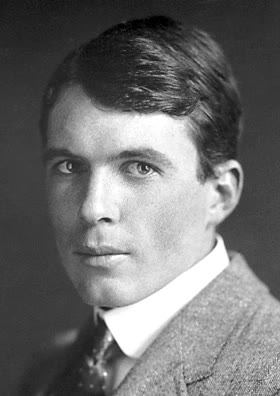
\includegraphics[width=\linewidth]{images/book4/bragg-wl.jpg}\par
{\footnotesize W. L. Bragg.}
\end{minipage}
\end{history}

\section{Exercises}

\begin{exercise}[$\star$]\label{exo:b3:x-ray-diffraction:1}
% ledger: lat:NaCl
For \ce{NaCl} ($a = \qty{564.06}{pm}$), compute $d_{111}$, $d_{200}$ and $d_{220}$.
\end{exercise}

\begin{exercise}[$\star$]\label{exo:b3:x-ray-diffraction:2}
% ledger: lat:Cu, xray:CuKa1
Copper is FCC with $a = \qty{361.50}{pm}$. With Cu K$\alpha_1$ ($\lambda = \qty{154.06}{pm}$),
compute $2\theta$ of its first two reflections, after naming them.
\end{exercise}

\begin{exercise}[$\star$]\label{exo:b3:x-ray-diffraction:3}
Which of the reflections 100, 110, 111, 200, 210, 211, 220 are present for a
cubic P, I and F lattice?
\end{exercise}

\begin{exercise}[$\star$]\label{exo:b3:x-ray-diffraction:4}
Give the reciprocal basis of a two-dimensional rectangular lattice of sides
$a$ and $b$, and draw the first reciprocal nodes.
\end{exercise}

\begin{exercise}[$\star\star$]\label{exo:b3:x-ray-diffraction:5}
% ledger: lat:W
A metal gives lines at $2\theta = 40.27$, 58.26, 73.20, 87.01 and \ang{100.66} with Cu
K$\alpha_1$. Index the pattern, find the lattice type and $a$.
\end{exercise}

\begin{exercise}[$\star\star$]\label{exo:b3:x-ray-diffraction:6}
% ledger: lat:KCl
A crystal of \ce{KCl} ($a = \qty{629.29}{pm}$) has a measured density of
\qty{1.99}{g/cm^3} (data of the exercise). Find $Z$.
\end{exercise}

\begin{exercise}[$\star\star$]\label{exo:b3:x-ray-diffraction:7}
The (200) line of a \ce{NaCl} nanopowder ($2\theta = \ang{31.70}$) is \ang{0.40} wide,
the instrument contributing nothing. Estimate the crystallite size.
\end{exercise}

\begin{exercise}[$\star\star$]\label{exo:b3:x-ray-diffraction:8}
\ce{CsCl} has \ce{Cs+} at $(0,0,0)$ and \ce{Cl-} at $(\frac12,\frac12,\frac12)$ in a P cell. With $f
\approx$ the number of electrons, compute $F_{100}$ and $F_{110}$ and the ratio of their
intensities (\omterm{def:b3:x-ray-diffraction:structure-factor}{structure factor} only). Why is \ce{CsCl} not body-centred?
\end{exercise}

\begin{exercise}[$\star\star$]\label{exo:b3:x-ray-diffraction:9}
Show that a C-centred lattice (extra node at $(\frac12,\frac12,0)$) makes the
reflections with $h + k$ odd absent.
\end{exercise}

\begin{exercise}[$\star\star\star$]\label{exo:b3:x-ray-diffraction:10}
Explain why the 1980s discovery of alloys whose diffraction patterns show sharp
spots with tenfold symmetry did not contradict the crystallographic
restriction, and what it changed in the definition of a crystal.
\end{exercise}

\begin{exercise}[$\star\star\star$]\label{exo:b3:x-ray-diffraction:11}
Show that in \textit{P}$2_1/c$ the \omterm{def:b3:x-ray-diffraction:space-group}{glide plane} makes the reflections $h0l$ with $l$
odd absent.
\end{exercise}

\begin{exercise}[$\star\star\star$]\label{exo:b3:x-ray-diffraction:12}
A pure enantiomer can never crystallise in a \omterm{def:b3:x-ray-diffraction:space-group}{space group} containing an
inversion centre, a mirror or a \omterm{def:b3:x-ray-diffraction:space-group}{glide plane}. Why? To which kind of \omterm{def:b3:x-ray-diffraction:space-group}{space groups} is
it restricted, and what does Friedel's law imply for determining its absolute
configuration?
\end{exercise}

% keep the heading with its problem box, which fills a page by itself
\clearpage
\enlargethispage{3\baselineskip}
\section{Problem: Which White Powder?}

\begin{problem}[{Weekend problem --- a powder pattern of an unknown cubic salt:
spacings, indexing, the lattice parameter and the identity of the salt, and the
size of its crystallites}]
\label{pb:b3:x-ray-diffraction:1}
% ledger: xray:CuKa1, lat:NaCl, lat:KCl, lat:KBr
An unknown white crystalline powder, known to be \ce{NaCl}, \ce{KCl} or \ce{KBr},
gives with Cu K$\alpha_1$ radiation ($\lambda = \qty{154.059}{pm}$) the lines (data of the
problem, computed for this exercise):
\begin{center}\small
\begin{tabular}{lcccccc}
\hline
$2\theta$ / degree & 28.342 & 40.512 & 50.178 & 58.632 & 66.380 & 73.692 \\
relative intensity & 100 & 92 & 38 & 20 & 61 & 49 \\ \hline
\end{tabular}
\end{center}
No other line appears between 20 and \ang{75}. Reference lattice parameters:
\ce{NaCl} \qty{564.06}{pm}, \ce{KCl} \qty{629.29}{pm}, \ce{KBr} \qty{658.47}{pm}. Molar masses:
K 39.1, Na 23.0, Cl 35.5, Br \qty{79.9}{g/mol}.

\medskip\noindent\textbf{Part I --- Spacings.}
\begin{enumerate}
  \item Compute $\theta$ and $d$ for the first line.
  \item Compute $d$ for all lines.
  \item Compute the ratios $\sin^2\theta/\sin^2\theta_1$.
  \item What series of integers do you find?
  \item Could the pattern be that of a primitive cubic lattice? With which $a$?
  \item For a primitive cubic lattice, which integer $N$ can never occur? Does
        the pattern tell the two interpretations apart so far?
\end{enumerate}

\medskip\noindent\textbf{Part II --- The real lattice.}
\begin{enumerate}[resume]
  \item All three candidates are F lattices. Index the lines with the F series.
  \item Deduce $a$ from the first line.
  \item Which candidate fits?
  \item For that salt, why are the all-odd reflections (111), (311) absent?
  \item Would \ce{NaCl} show (111)? \ce{KBr}?
  \item Explain why the primitive interpretation of Part I is a trap.
\end{enumerate}

\medskip\noindent\textbf{Part III --- Density and contents.}
\begin{enumerate}[resume]
  \item How many formula units does the cell contain?
  \item Compute the density from the cell.
  \item Give the coordination number of each ion.
  \item Compute the shortest K--Cl distance.
  \item What reflection would appear first above \ang{75}?
  \item Why are intensities less useful than positions for identifying a phase?
\end{enumerate}

\medskip\noindent\textbf{Part IV --- Refinement and crystallite size.}
\begin{enumerate}[resume]
  \item Why is the lattice parameter best computed from a high-angle line?
  \item Compute $a$ from the (420) line.
  \item The (420) line is \ang{0.25} wide in $2\theta$ (instrumental width
        negligible). Estimate the crystallite size.
  \item Would a crystallite size of \qty{1}{\micro m} broaden the line measurably?
  \item State the result: the lattice parameter refined from the (420) line, and
        the identity of the powder.
\end{enumerate}
\end{problem}
